\documentclass[a4paper, 10pt, final, garamond]{book}
\usepackage{cours-preambule}
\graphicspath{{./figures/}}

\makeatletter
\renewcommand{\@chapapp}{Contr\^ole de connaissances}
\makeatother

% \toggletrue{student}
% \toggletrue{corrige}
\renewcommand{\mycol}{black}
% \renewcommand{\mycol}{gray}

\begin{document}
\setcounter{chapter}{28}

\settype{enon}
\settype{solu}

\chapter{Solides cristallins\ifstudent{~(15')}}

\begin{enumerate}[label=\sqenumi]
	\item[n]{11} %
	\textbf{Dessiner} la maille cubique faces centrées et donner le lieu de
	tangence. Réaliser sa caractérisation complète (population, coordinence, rayon
	atomique, compacité, masse volumique~: \textbf{définition} puis formule).
	\smallbreak
	\noindent
	\begin{isd}[righthand ratio=.24, interior hidden]
		\begin{itemize}
			\item[b]{Population}: \psw{8 atomes sur les sommets et 6 sur les faces,
				soit
				\[
					N \stm{=} 8 \times \frac{1}{8} + 6 \times \frac{1}{2} = 4
				\]
			}%
			\vspace{-15pt}
			\item[b]{Coordinence}: \psw{chaque atome voit les voisins sur \textbf{les
					petites diagonales des faces} \pt{1}. On a donc une coordinence de
				\textbf{12}. \pt{1}}
			\item[b]{Rayon atomique}: \psw{on a tangence \textbf{sur les petites
					diagonales}, soit
				\[
					r + 2r + r \stm{=} a \sqrt{2} \Lra \boxed{2r \sqrt{2} = a}
					\quad \pt{1}
				\]
			}%
		\end{itemize}
		\tcblower
		\begin{center}
			\sswitch{
				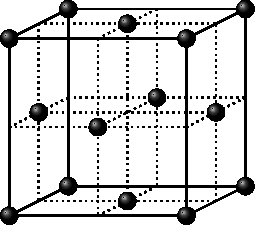
\includegraphics[width=.8\linewidth, draft=true]{maille_CFC}
			}{
				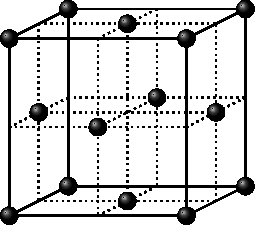
\includegraphics[width=.8\linewidth]{maille_CFC}
			}
			\sswitch{
				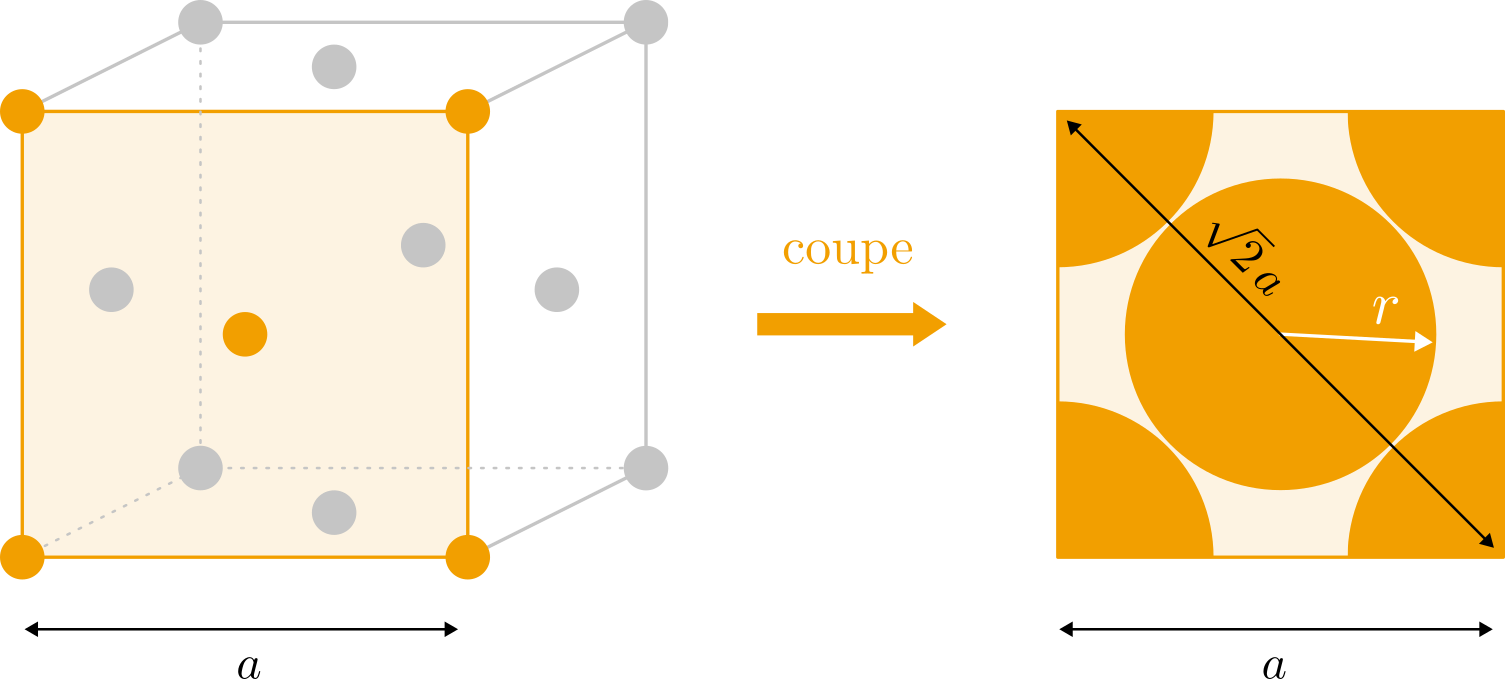
\includegraphics[width=\linewidth, draft=true]{maille_CFC_rayon}
			}{
				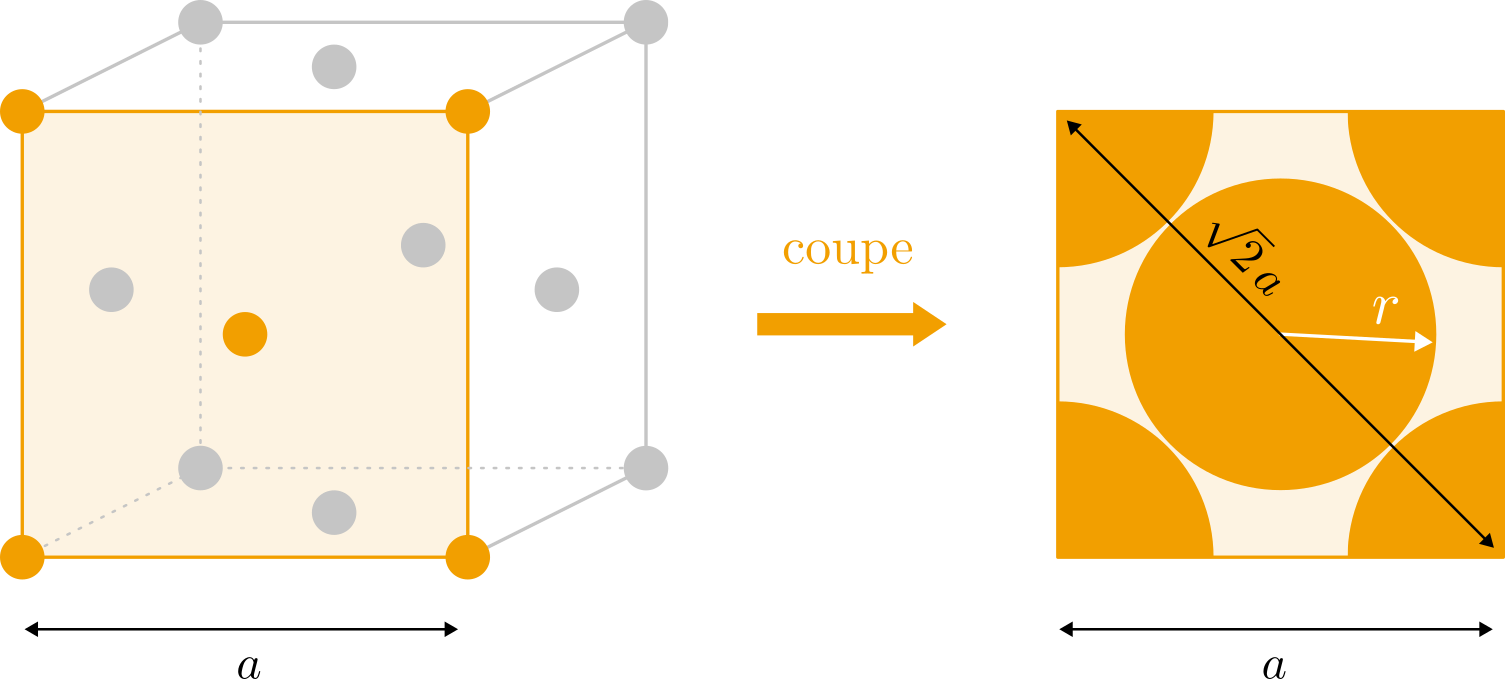
\includegraphics[width=\linewidth]{maille_CFC_rayon}
			}
			\vspace{-15pt}
			\captionof*{figure}{Maille CFC~\protect\pt{1}\psw{+}\protect\pt{1}}
		\end{center}
	\end{isd}
	\vspace{-30pt}
	\begin{itemize}
		\item[b]{Compacité}:
		\leavevmode\vspace*{-30pt}\relax
		\psw{%
			\begin{gather*}
				C \stm{=}
				\frac{NV_1}{V} =
				\frac{\bcancel{4} \times \frac{\bcancel{4}}{3}\pi \cancel{r^3}}
				{\bcancel{16} \sqrt{2}\cancel{r^3}}
				\Lra
				\boxed{C \stm{=} \frac{\pi}{3 \sqrt{2}} \approx \num{0.74}}
			\end{gather*}
		}%
		\item[b]{Masse volumique}:
		\leavevmode\vspace*{-25pt}\relax
		\psw{%
			\begin{gather*}
				\rho \stm{=} \frac{\text{masse des motifs}}{\text{volume de la maille}}
				\Lra
				\rho \stm{=} \frac{4M}{\Nc_A \times a^3}
			\end{gather*}
		}%
		\vspace{-15pt}
	\end{itemize}
	\vspace*{\fill}
	\item[n]{11}
	Justifier alors l'existence des sites interstitiels. Donner \textbf{sans
		schéma} les positions et la population des sites T et O de la structure CFC,
	et déterminer leurs habitabilités en fonction de $r$ le rayon des sphères
	principales.
	\smallbreak
	\begin{itemize}
		\item[b]{Justification}:
		\psw{%
			Même dans les mailles compactes, il reste du vide et toutes les sphères ne
			se touchent pas~: on peut insérer de \textbf{plus petites entités}
			entre les entités principales d'une CFC.~\pt{1}
		}%
	\end{itemize}
	\smallbreak
	\begin{isd}[sidebyside align=top]
		\tcbsubtitle{\fatbox{\textbf{Sites tétraédriques}}}
		\begin{itemize}
			\item[bl](\pt{1}){Position}: \psw{au centre des petits cubes d'arête $a/2$.}
			\item[bl](\pt{1}){Population}: \psw{il y a 8 petits cubes et les entités sont dans
				le volume, soit $N_T = 8$.}
			\item[bl](\pt{1}){Habitabilité}:
			\psw{%
				On a tangence \textbf{sur la moitié de la grande diagonale du petit
					cube}~:
				\begin{DispWithArrows*}[fleqn, mathindent=5pt]
					r + r_T \stm{=} \frac{a \sqrt{3}}{4}
					&\Lra
					\boxed{r_T = \frac{a \sqrt{3}}{4} - r}
					\Arrow{$a = 2r \sqrt{2}$}
					\\\Lra
					\Aboxed{r_T &\stm{=} \left( \sqrt{\frac{3}{2}} - 1 \right)r \approx \num{0.225}r}
				\end{DispWithArrows*}
			}%
			\vspace{-15pt}
		\end{itemize}
		\tcblower
		\tcbsubtitle{\fatbox{\textbf{Sites octaédriques}}}
		\def\lspace{13}
		\begin{itemize}
			\item[bl](\pt{1}){Position}: \psw{au centre de chaque arête et 1 au
				centre.}
			\item[bl](\pt{1}){Population}: \psw{12 arêtes et 1 centre, soit $N_O =
					1+12 \times \frac{1}{4} = 4$}
			\item[bl](\pt{1}){Habitabilité}:
			\psw{%
				On a tangence \textbf{sur une arête}~:
				\begin{DispWithArrows*}[fleqn, mathindent=5pt]
					2(r + r_O) \stm{=} a
					&\Lra
					\boxed{r_O = \frac{a}{2} - r}
					\Arrow{$a = 2r \sqrt{2}$}
					\\\Lra
					\Aboxed{r_O &\stm{=} \left( \sqrt{2} - 1 \right)r \approx \num{0.414}r}
				\end{DispWithArrows*}
			}%
		\end{itemize}
	\end{isd}
\end{enumerate}
\vspace*{\fill}
\ifstudent{
	\begin{tikzpicture}[remember picture, overlay]
		\node[anchor=north west, align=left]
		at ([shift={(1.4cm,0)}]current page.north west)
		{\\[5pt]\Large\bfseries Nom~:\\[10pt]\Large\bfseries Prénom~:};
		\node[anchor=north east, align=right]
		at ([shift={(-1.5cm,-17pt)}]current page.north east)
		{\Large\bfseries Note~:\hspace{1cm}/20};
	\end{tikzpicture}
}
\end{document}
